 %----------------------------------------------------------------------------------------
%	PACKAGES AND OTHER DOCUMENT CONFIGURATIONS
%----------------------------------------------------------------------------------------

\documentclass[twoside]{article}

\usepackage{lipsum} % Package to generate dummy text throughout this template

\usepackage[sc]{mathpazo} % Use the Palatino font
\usepackage[T1]{fontenc} % Use 8-bit encoding that has 256 glyphs
\linespread{1.05} % Line spacing - Palatino needs more space between lines
\usepackage{microtype} % Slightly tweak font spacing for aesthetics

\usepackage[hmarginratio=1:1,top=32mm,columnsep=20pt]{geometry} % Document margins
\usepackage{multicol} % Used for the two-column layout of the document
\usepackage[hang, small,labelfont=bf,up,textfont=it,up]{caption} % Custom captions under/above floats in tables or figures
\usepackage{booktabs} % Horizontal rules in tables
\usepackage{float} % Required for tables and figures in the multi-column environment - they need to be placed in specific locations with the [H] (e.g. \begin{table}[H])
\usepackage{hyperref} % For hyperlinks in the PDF

\usepackage{lettrine} % The lettrine is the first enlarged letter at the beginning of the text
\usepackage{paralist} % Used for the compactitem environment which makes bullet points with less space between them

\usepackage{abstract} % Allows abstract customization
\renewcommand{\abstractnamefont}{\normalfont\bfseries} % Set the "Abstract" text to bold
\renewcommand{\abstracttextfont}{\normalfont\small\itshape} % Set the abstract itself to small italic text

\usepackage{titlesec} % Allows customization of titles
\renewcommand\thesection{\Roman{section}} % Roman numerals for the sections
\titleformat{\section}[block]{\large\scshape\centering}{\thesection.}{1em}{} % Change the look of the section titles
\titleformat{\subsection}[block]{\normalsize}{\thesubsection.}{1em}{} % Change the look of the section titles

\usepackage{fancyhdr} % Headers and footers
\pagestyle{fancy} % All pages have headers and footers
\fancyhead{} % Blank out the default header
\fancyfoot{} % Blank out the default footer
\fancyhead[C]{CA640 $\bullet$ 21/Nov/14 $\bullet$ Pr�cis Assignment} % Custom header text
\fancyfoot[RO,LE]{\thepage} % Custom footer text

\usepackage{natbib}
\bibliographystyle{agsm}

\usepackage{graphicx}
\usepackage{float}


%----------------------------------------------------------------------------------------
%	TITLE SECTION
%----------------------------------------------------------------------------------------

\title{\vspace{-15mm}\fontsize{24pt}{10pt}\selectfont\textbf{Paper Pr�cis: Creating a Shared Understanding of Testing Culture on a Social Coding Site}} % Article title

\author{
\large
\textsc{Anthony Troy }\\[2mm] 
\normalsize \href{mailto:anthony.troy3@mail.dcu.ie}{anthony.troy3@mail.dcu.ie | 14212116} \\
\vspace{-5mm}
}
\date{}

%----------------------------------------------------------------------------------------

\begin{document}

\maketitle % Insert title

\thispagestyle{fancy} % All pages have headers and footers

%----------------------------------------------------------------------------------------
%	Disclaimer, Pr�cis & ABSTRACT
%----------------------------------------------------------------------------------------
\renewcommand{\abstractname}{\vspace{-\baselineskip}}
\begin{abstract}
\noindent \textbf{Disclaimer}: Submitted to Dublin City University, School of Computing for module CA640: Research Skills, 2014/2015. I hereby certify that the work presented and the material contained herein is my own except where explicitly stated references to other material are made.
\end{abstract}

\vspace{-7mm}

\renewcommand{\abstractname}{\vspace{-\baselineskip}}
\begin{abstract}
\noindent  \textbf{Basing Paper}: R. Pham, L. Singer, O. Liskin, F. Figueira Filho, and K. Schneider. Creating a shared understanding of testing culture on a social coding site. In Proceedings of the 2013 International Conference on Software Engineering, ICSE 2013, pages 112-121, Piscataway, NJ, USA, 2013. IEEE Press.
\end{abstract}

\vspace{1mm}
\renewcommand{\abstractname}{Abstract}
\begin{abstract}
\noindent 
Software engineering is inherently collaborative, at the team, project and community levels. However many project
owners battle with establishing and communicating a testing culture that is appropriate for their project's needs.
Transparent software environments such as Github incorporate social media features to make work more visible. 
Previous research forwards that this transparency influences the behaviour of developers. Our basing paper
extends upon those findings to investigate how the increased transparency found on GitHub influences testing 
behaviours.\par
Derived from interviewing active GitHub users, both project owners and developers, our basing paper 
suggests several strategies that software teams can use to positively influence the testing behaviour in their projects. 
Additionally, it is found that project owners on GitHub are often not aware of these strategies. This research reports
on the difficulties and risks which this causes and suggests guidelines for developing a sustainable testing culture.

\end{abstract}

%----------------------------------------------------------------------------------------
%	ARTICLE CONTENTS
%----------------------------------------------------------------------------------------

\begin{multicols}{2} % Two-column layout throughout the main article text

\section{Introduction}

Like many fields that rely closely on collaboration
and coordination, Software Engineering is rapidly transforming. The emergence of
social media sites --- both general and those specifically created for software 
developers --- has resulted in a paradigm shift in the field; developers 
can now connect with, provide help to, collaborate with, and learn from one another 
with ease \citep{Storey}. \par
By virtue social media sites provide a high degree of social transparency, 
making freely available the "social meta-data" around information exchange 
\citep{Stuart}. \citet{Dabbish} forwards that the transparency GitHub provides
influences the behaviour of software developers. Our basing paper investigates 
how testing behaviour is influenced by such social coding sites. \citet{Pham},
the paper author, poses that there exists no previous work on this topic and that
"if social coding sites can influence the testing behaviour of developers, they
might also have an impact on the progress of software development projects 
and their resulting projects". \par 
\setlength{\parskip}{0em} % hack 
In accordance with our basing paper, this 
pr�cis is structured as follows. In section II, we describe some related works
around this topic, furthering from this section III outlines the respective study 
undertaken. Section IV discusses the emerged findings and section V concludes 
this pr�cis.

%------------------------------------------------

\section{Related Work}

This section outlines existing research as regards open source software 
(OSS) development, testing activities and social coding sites.
\par

\textbf{\textit{Testing Practices:}} a wealth of research has been conducted around
testing practices in OSS projects. For example, \citet{Michlmayr} conducted study 
that investigated the quality-related processes in a diverse set of open source projects. 
\citet{Greiler} specifically investigate testing practices in the Eclipse Plug-In community. 
\par

\textbf{\textit{Social coding sites}} have been subject to significant research efforts 
in recent years.
\citet{Stuart} forwards a conceptual framework on the effects of social 
transparency on behaviour. \citet{Singer} investigates "developer profile aggregators" 
that combine developer activities from social coding sites and other social media. 
\citet{Dabbish} explores the relationship between social transparency and developer 
behaviour on GitHub.
\par

\textbf{\textit{OSS development}} projects are open in nature and thus
 the area of OSS has been heavily researched.  
\citet{Bonaccorsi} explores the motivations of both developers and software companies 
that participating in OSS development. \citet{Mockus} forwards an OSS development 
process model based on the Apache Web Server project. \citet{Crowston} explicitly
study bug fixing processes in OSS development.  \citet{Dagenais} 
study API documentation processes and how developers employ them to learn 
in OSS environments. \citet{Stewart} demonstrate how developer ideology in 
an OSS project influence its effectiveness. 

\par
\textbf{\textit{Coordination and awareness}} within teams are the subject 
of some CSCW research focused on software development. For example, 
\citet{Begel} report on a newsfeed system that increases project 
awareness. 
\citet{Souza} investigate which actions should be 
presented to whom in such feeds.

\par
While most of these studies report on concepts that are also found in our basing paper, 
Pham's (2013) contribution extends upon them by specifically exploring the related 
influences on testing, which exist "due to (the) peculiarities of social coding sites, such 
as the high degree of social transparency, remarkably low barriers, and a high 
centralisation and integration of tools and interfaces".

%------------------------------------------------

\section{Study Design}

Our basing paper employs a general research method, Grounded Theory \citep{Anselm}, to explore how testing is carried out on GitHub and investigate how increased social transparency influences testing behaviour. 
Pham emphasised on two groups of people:
\begin{enumerate}
	\item project owners, who receive pull requests
	\item contributors who send them
\end{enumerate}

\subsection{Research Questions}

For the initial data collection phase a survey was designed which included five questions to better help "understand how testing practices evolve based on the interaction between contributors and project owners on social coding sites" \citep{Pham}. This questionnaire (Q1) analysed the following topics:
\begin{itemize}
	\item how project owners assess incoming contributions
	\item internal and external motivations for engaging in testing efforts
	\item the challenges and risks related to testing
	\item how developers code with those challenges and risks
	\item	the impact of participating on social coding projects has on testing practices
\end{itemize} 

\subsection{Procedure}

Grounded Theory \citep{Anselm} involves continuous data collection accompanied with periodic pauses for analysis. Accordingly, our basing study was conducted in three incremental phases of analysis. Pham first enlisted a diverse sample population though inviting active GitHub users belonging to popular OSS projects and random recently active GitHubs users. The first phase sought to understand which testing-related norms and conventions exist on Github through broadly asking participants to outline their testing process in one of their public projects. The findings from this phase posed that projects which featured extensive collaboration between developers would demand more elaborate testing approaches. Additionally, these findings indicated that most decisions regarding testing were made when pull requests were sent and received, hence when people had to coordinate and negotiate their cooperation.
\par
Subsequently, the second phase of the analysis involved refining the target population to be "active users who used the collaboration features of GitHub" \citep{Pham}. Such was achieved by inviting the sample pool to take the first questionnaire (Q1), whereby the questionnaire responses made it possible to distinguish those users that had been collaboratively active and their approaches from testing contributions. Furthering from this, the refined target population were invited to a round of semi-structured interviews exploring participant's testing practices and values. Several common themes emerged from interviews:

\begin{enumerate}
	\item The social network features, fork and pull request mechanisms, and integration of numerous tools result 		in a GitHub-specific process for sending and receiving contributions.
	\item GitHub tools and social features lower the barriers for engagement in software projects.
	\item GitHub integrates many tools into the project context and centralizes many interactions and notifications
		among project participants.
	\item GitHub provides increased social transparency that al-
		lows its users to see the identity, actions, and com- munications between users
\end{enumerate}

In the last phase, a final questionnaire (Q2) was sent to random GitHub users for quantitative validation of Pham's findings, this is outlined in section V.

%------------------------------------------------

\section{Findings}

\textbf{\textit{Interaction on GitHub with Regard to Testing:}} The interview process presented several common steps in the GitHub contribution process. After receiving a pull request (PR), a project owner manually reviews the contribution and assess it by different
aspects. Following such, they merged the PR into a testing branch and resolved conflicts manually. If a test suite existed, owners ran it to check whether or not this contribution passed. Finally, the contribution was merged into the main branch of the project. 
\par
It emerged that many factors that were taken into consideration by owners when assessing contributions, such are as follows: 
\begin{itemize}
\item \textbf{Contribution Size:} the perceived size of the changes highly influenced the project owner's need for tests.
\item \textbf{Developer Trust:} owners treated incoming PRs differently depending on whether they trusted the contributing developer.
\item \textbf{Contribution Type:} owners had different testing approaches for contributions that introduced a new feature and contributions that changed existing code. The former were requested to include test whereas the latter caused project owners to check whether or not the changed code was already covered by existing tests. 
\end{itemize} 
\par

\textbf{\textit{Motivations for Demanding \& Delivering Tests:}} Project owners' reasons for demanding tested contributions were manifold. Maintaining clean and well documented code reduced the subsequent support effort, according to one project owner. 

Some project owners perceived tests as a form of documentation of how to use the contributed feature. Another project owner requested contributors to provide test cases of how they needed the software to behave, so he could merge these into the existing test suite for future regression testing. In this case, tests were used for communicating requirements.
An external motivator was the impression of acting as a role model when working on a testing-related project. Several users reported to feel obliged to perform proper quality assurance for projects with a domain related to testing ? e.g. a testing framework or a continuous integration server.
In interviews with contributors, different motivations for including tests in a pull request on one?s own initiative emerged. Some interviewees said they explicitly added tests that highlight the value of their contribution to the project owner: these tests failed with the old version of the software in question, but passed when the contribution was applied.
The existence and prominent placement of tests gave contributors the impression of informal project guidelines; thus they felt obligated to add their own tests. ?[There were no guidelines set up], not so much formally, but it was pretty clear how it was supposed to be tested and there was already an existing spec file [...] with a pretty substantial list of tests? [FI17]
Similar to a project owner perceiving oneself as a role model when working on a testing-related project, contributors felt an implicit demand for tested pull requests in such domains. In other instances, this obligation also resulted from customs rooted in the community of the technology used. Often, Ruby developers tested their contribution by default.

\subsection{Challenges and Risks}

This section discusses the challenges and risks we found to arise when engaging with projects on GitHub (RQ 2).
Interviewees saw an urgent need for automatic tests in their projects. This need was felt very strongly, as there are a lot of contributors on GitHub which are often only marginally engaged, i.e., there is a large group of developers in the periphery. Therefore, a lot of contributions need to be managed which interviewees reported could not be done using manual tests ? simply for reasons of scale. ?a lot of people are contributing to [the project] and quality control is becoming more and more important to us. Automated testing is the only way to get that? [FI7] To achieve automated testing, project owners were in many cases looking for tests when they received pull requests from contributors (cf. the previous section).
Because there is a constant flux of contributors, and developers new to a project are not yet accustomed to its testing culture, they have to learn it anew. This takes time and effort. If a project fails to communicate testing culture efficiently and effectively, or sets barriers that are too high for first-time contributors, it can struggle to create such a culture. For example, if new contributors cannot easily find existing tests in a project, they will not be able to write any of their own for their contributions. ?When I first started contributing to [the project], they did not actually have a test suite which made shipping them tests fairly difficult? [FI20]
Several project owners reported that their projects were struggling with creating the required testing culture. The pull requests they received would often not include any tests by default. One issue they saw was the voluntary nature of
open source contributions: they could not simply require well- tested contributions. Developers who had sent a valuable pull request might be alienated if project owners rejected their contributions due to a lack of tests. ?We have a project, where we don?t have the culture, it is difficult and people are volunteers, we can?t just enforce it on the project. You have to try to incubate it into the project.? [FI7]
Another reason why creating a robust testing culture is so difficult could be the lack of experience on the side of the contributors. ?We have a lot of people ramping up to the team every time. So, we have a big rotation. So new people don?t understand what is a quick build, what is the regression, what is isolated, ... and they don?t understand how to write tests for each of those suites.? [L4]
Two of GitHub?s greatest strengths ? low barriers to contribution, combined with tight integration of related tools and services ? are related to another challenge that interviewees mentioned. In terms of testing, there are no integrated tools provided by GitHub that might lower some testing-related barriers, e.g. for setting up a server for continuous integration. Even though this is starting to be supported by Travis CI5, this was not yet commonly used amongst the interviewed population. One interviewee even mentioned that ?github its such an easy-to-use-tool that it makes writing unit tests seem like extra time for most people.? [R16]

\subsection{Coping with Challenges}

In this section, we report how interviewees coped with the testing-related challenges on GitHub (RQ 3).
As described in the previous section, scalability reasons drive project owners towards automated tests. However, man- ually merging each pull request into a testing branch and running regression tests with a test suite of automated tests remained a tedious task. Some interviewees resorted to an automated continuous integration (CI) service, such as Travis CI or Jenkins. Such a service frees the project owner of several manual steps: when a pull request is received, a program merges the contribution into a testing branch, runs the existing test suite, and notifies the project owner as well as the contributor of the results.
Project owners developed different strategies to establish a common understanding of testing requirements and handling untested pull requests. Due to the voluntary nature of GitHub (c.f. previous section), some project owners simply resorted to writing tests themselves or thankfully requesting ? instead of demanding ? further tests, as this leaves the contributor the option to decline.
Lowering the barriers and making it easier to provide tests was another strategy, for example by introducing a testing framework with a suitable explanation of its usage. Other project owners provided easy access to learning resources and actively supported contributors who showed difficulties in writing tests: pointing contributors to tutorials, suitable examples in an existing test suite, or actively teaching them
This was beneficial as contributors were convinced of the need for tests and included tests on their own in subsequent pull requests. ?[...] I can point them to one of the existing tests. �Check this one, it is really similar to what you need�, and in most cases it?s enough. Sometimes, [...] I do Skype conferences with screen sharing where I can explain, show.? [FI4]
A passive strategy for communication testing requirements was to make it more obvious that testing was indeed desired by giving the impression that testing was a customary in one?s project. Some interviewees said that they tried to lead by example and tried to make testing visible in the project, hoping to engage contributors in testing. Another strategy was to display testing signals. For example, every project using Travis CI may add a badge to its profile page. This informs a potential contributor that continuous integration is regularly performed. ?if you see that image, it immediately rings the bell that there is continuous integration in this project, and as such, there is some kind of automated testing.? [FI6]

\subsection{Impact of Social Coding Sites on Testing Practices}

This section investigates the impact of engaging with a social coding site on testing practices (RQ 4).
During our research, we encountered different levels of lowering the effort for testing. One interviewee suggested that in his perception, projects using behavior driven development (BDD) and concentrating on testing primarily the main use cases provided these low barriers to entry. This allowed those projects to deliver results very fast, which impressed other developers. Those projects were also very good at communicating their culture in social media, e.g. via blog posts advocating their testing culture. This combination, the interviewee said, would lead to the described behavior being adopted at a fast rate and thus spreading through GitHub. He saw this development critically however, as possibly important edge cases were ignored until they became apparent.
A more extreme case of lowering the barrier for contribu- tions was simply to defer testing to a later stage of the project. An interviewee said that in his experience, younger projects needed to gain traction in the present. Obtaining external contributions was regarded to be more important than quality assurance measures. However, such projects would need to pay back this accumulated technical debt in the future.
Interviewees told us that effectively communicating a project?s testing culture would lead to contributors adopting that culture more rapidly and in greater numbers. We spoke to several developers who had experiences in multiple projects with different communication strategies. According to them, better communication of testing culture leads to more pull requests containing tests, and therefore to projects that were tested better. Testing guidelines and actively communicating to contributors what kind of tests were required helped getting more contributors to provide tests with their pull requests. Providing guidelines on contributing or providing dedicated testing tutorials removed uncertainties in contributors about how to participate correctly. This way, the barrier of having to ask was removed. One interviewee expressed that knowing
a project?s testing culture and adhering to it would make him and his peers feel proud, further helping the project?s testing culture to be adopted. However, the reverse was also mentioned: if a project did not communicate anything about its norms and requirements regarding testing, new contributors would simply assume that no tests had to be written and consequently submit pull requests not containing any.
Some interviewees mentioned that testing culture ? and communicating it ? could even be ingrained not only in a single project, but in a whole infrastructure community (c.f. section V-B). According to these interviewees, in the Ruby community it was taken for granted that blog posts, screen casts, and tweets from popular developers often talked about testing practices that were regarded as proper in that community. This is a form of communicating a testing culture ? in this case however, in a much larger realm than that of one or more GitHub projects.
Interviewees reported several examples where direct ex- changes on GitHub helped diffusing testing culture. For example, one project owner reported that his project started using the Travis CI service when it received a pull request that added a Travis CI configuration file. ?I received a Travis CI config [in a pull request]. I did not know this service before and someone send me a config for Travis and this is how I came to use it? [FI19]
Travis CI, in turn, also arranges for low barriers and easy communication of testing culture. As described in section V-D, the Travis CI badge is perceived as a signal that com- municates the use of certain practices.
However, employing a continuous integration service with an extensive test suite may create a false sense of security: one interviewee reported to use the positive result of running his existing test suite as a sufficient confirmation of a con- tribution?s correctness. He usually simply merged such pull requests without requesting any additional tests specific to these contributions.
A key instrument for project owners wishing to create and nurture their project?s testing culture was to provide existing tests and a testing infrastructure that was easy to set up (c.f. section V-D). Interviewees reported this to lower the barrier to accommodate to the project?s culture. They would just need to fork the project, execute a shell command, and have the existing tests running. Interviewees took this as an opportunity to run regression tests, thus trying to make sure that their contribution did not break anything. This increased their confidence in the correctness of their own code and lowered the barrier of contributing. Some interviewees also said that just having a test suite would communicate certain values regarding testing, helping them understand the project?s testing culture, norms, and conventions. Providing publicly available tests brought by another advantage: contributors heavily used existing tests as a source for education and examples for their own test cases. ?there were some tests surrounding some quite similar functionality in the source, so I basically copied and modified these tests to test the functionality that I added.? [FI20] One recurring theme was that communicating of testing culture better and lowering barriers in a project promote explo- ration and experimentation for new contributors. Interviewees claimed that this, in turn, often leads to developers becoming more familiar with a project?s testing culture, making it easier for them to provide their own tests. For example, a project with a CI server that provided fast feedback on tests was said to support experimentation ? after all, problems would be easily visible, giving experimenting developers more confi- dence. Some interviewees mentioned that experimentation was supported not only by a project?s deliberate efforts, but also by the chosen programming language and the available libraries.
Interviewees claimed that the number of volunteer contri- butions increased since moving their projects to GitHub. They attributed this to the low barriers to entry and the resulting exposure to a larger number of developers. An employee of a company that develops open and closed source projects told us that many GitHub contributors find bugs, provide tests, and send them bug fixes. This, he claimed, enabled the company?s paid developers to concentrate on larger issues, such as creating new features.
To a greater extent, interviewees reported that the public na- ture of software development on GitHub leads to an improve- ment of testing practices. Some of them were companies that used the exemplary testing practices in their public projects as an advertisement for the high quality of their development services. Indeed, one employee of such a company confided that testing was less important in the company?s internal projects, as they did not serve as such advertisements.
We heard similar reports from open source projects not backed by companies. Core members of such projects were concerned about the project?s reputation ? how the project was perceived by the community. They believed that proper testing would lead to higher quality code, which in turn would be received better by others. ?we need to have a more substantial testing framework because it?s [...] a significant indicator of code quality in the community. If you don?t have good tests then people start to suspect that your code may not be any good either.? [FI17]
On the side of the contributors, one interviewee reported that having contributed to a high-profile project in which tests are mandatory would help him find work. Indeed, that was his only reason for contributing.
Our findings show that several mechanisms and processes used on GitHub may help projects become better tested. Project owners help new contributors get acquainted with a project?s culture and make it easy for them to get up and running technically. However, this does not only affect regular contributors that can be productive faster. Drive-by commits ? as an interviewee called them ? are small changes that do not require a prolonged engagement with a project, yet provide some value for it. Developers providing such changes would not always be actively interested in a project, but might have stumbled upon it when browsing GitHub. Then, when they had found, for example, a spelling error or a missing translation, they would make a quick correction and forget the
project again. GitHub?s integration and low barriers seemingly streamline this process and might lead to GitHub having a very long tail of many small contributions.
%------------------------------------------------
\section{Validating Findings}

This section poses striking results from the final questionnaire (Q2) which was used to validate core statements of Pham's findings. The according results are summarised in Table I, where C  illustrates statements about contributors and PO about project owners. 
For each question, we presented the participant with a Likert scale of five items ranging from ?I do not agree at all? to ?I strongly agree.?. These Likert items are represented in the diagrams on the X- axis with disagreement being on the left and agreement being on the right hand-side. The middle bar represents the neutral item. The number of answers accumulated for each Likert item is marked on the Y-axis. The grey bar is the median.
\begin{table}[H]
  \centering
  	\caption{Result of final questionnaire (Q2)}
	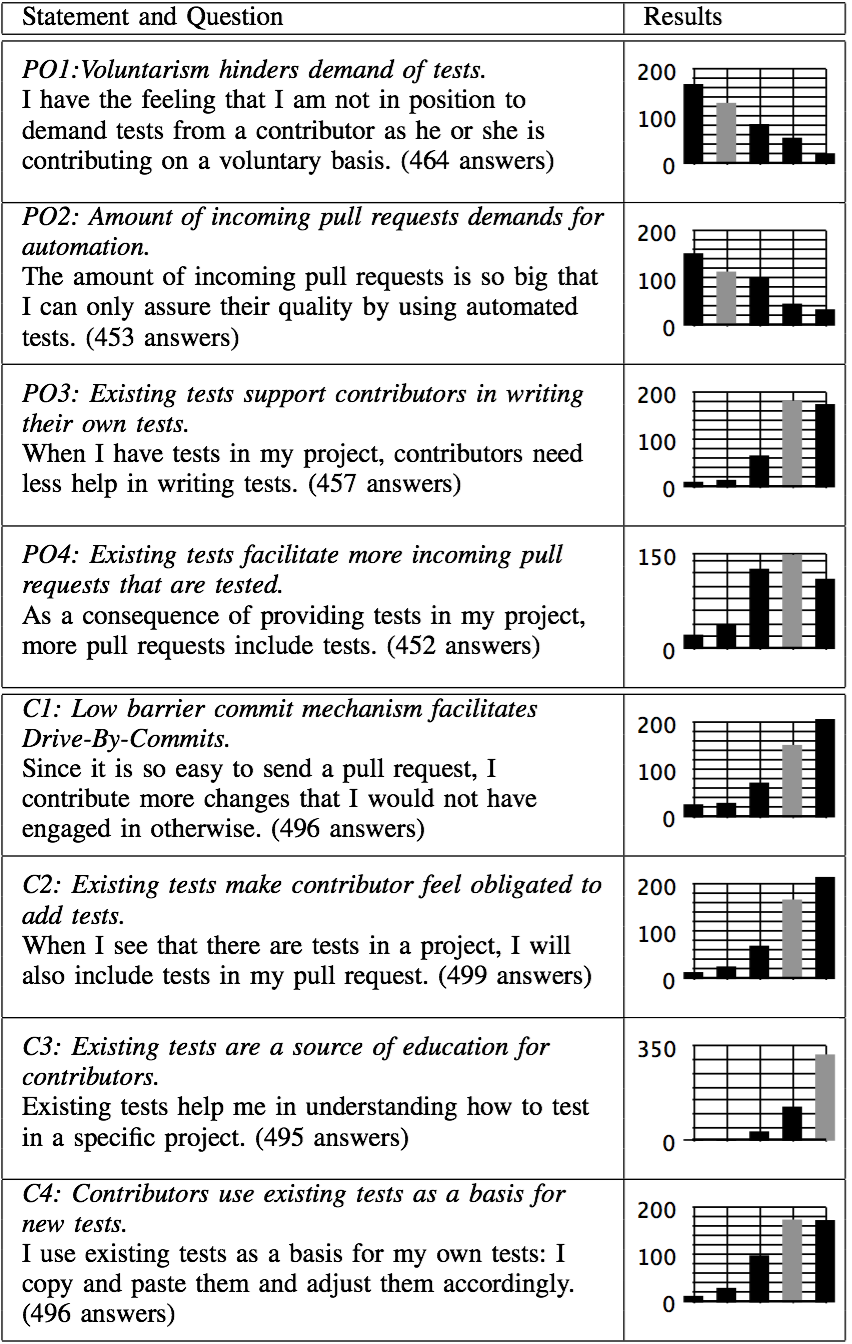
\includegraphics[width=77mm, height=150mm]{qa2.png}
\end{table}


The questionnaire required the participant to take both the perspective of a project owner and a contributor. 39\% of our participants would receive pull requests at least a few times per week (daily: 16\%) and 27\% send pull requests at least a few times per week (daily: 6\%). Even though several interviewees mentioned voluntarism as a hindering factor, the questionnaire did not validate this (PO1). Personal traits such as modesty and humility of the requester as well as value given to the contribution may be influencing factors. Similarly, most of the participants did not agree to feel a need for automation (PO2). However, as some interviewees mentioned, this need may depend on the size and popularity of the project in question. As popularity grows, the amount of incoming pull requests increases. As both samples were randomly invited, but ultimately self-selected, variations in populations might attribute for this dissonance.
Project owners agree that providing tests in one?s project lowers the support effort regarding testing by contributors (PO3). Appropriately, contributors heavily rely on existing test cases when creating their own. They use these to learn how testing is done in a specific project (C3) and, lastly, even copy existing tests and use them as a basis for new tests (C4). With tests in place, contributors feel obligated to add their own tests and seem to comply with this implicit demand (C2).

%------------------------------------------------

\section{Conclusions and Outlook}
When hosting a project on a social coding site such as GitHub, project owners interact with external contributors with varying knowledge and values regarding testing. Communi- cating a project?s testing culture to such a population is an important, yet difficult task.
Our study reports on the influences of GitHub?s peculiarities on testing practices ? especially its high degree of social transparency, low barriers, and high degrees of integration and centralization. We present insights about the contribution process on GitHub and show how project owners assess pull requests with regard to testing. We found several testing- related challenges that members of GitHub face ? and the strategies they have developed to cope with them, helping them create a shared understanding of a project?s testing culture.
Developers on social coding sites can use our findings to gain insights into issues contributors may face and the strate- gies that can be used to handle them. Software development organizations may take our contributions as inspiration for basing their own testing-related communication strategies on.
This research is an exploratory first step to gain an under- standing of the testing norms, challenges, and strategies on social coding sites. It is a starting point for informed, in-depth investigations into several of the issues raised in our study.

%----------------------------------------------------------------------------------------
%	REFERENCE LIST
%----------------------------------------------------------------------------------------

\bibliography{article_2}

%----------------------------------------------------------------------------------------

\end{multicols}

\end{document}
